

%%%%%%%%%%%%%%%%%%%%%%%%%%%%%%%%%%%%%%
%
% General TODO:
%  - fix images' size
%  - improve style of code/identifier
%  - references / bibliography
%
%%%%%%%%%%%%%%%%%%%%%%%%%%%%%%%%%%%%%%

\documentclass{article}

\usepackage{graphicx}
\usepackage[usenames,dvipsnames,svgnames,table]{xcolor}
\usepackage[utf8]{inputenc}
\usepackage[T1]{fontenc}


%%%
% Commands

\newcommand{\id}[1]{\mbox{\textsc{#1}}}
\newcommand{\path}[1]{\mbox{\texttt{#1}}}

\newcommand{\TODO}[1]{\texttt{\textcolor{YellowOrange}{(#1)}}} % for inline TODO

%
%%%

\title{Large-scale Information Extraction from Neuroscientific Literature}
\date{Spring 2015}
\author{Marco Antognini}

\begin{document}

\maketitle

Master Semester Project under the supervision of:
Jean-Cédric Chappelier \&
Renaud Richardet
Artificial Intelligence Laboratory LIA - EPFL

\pagenumbering{gobble}
\newpage
\pagenumbering{arabic}


\tableofcontents
\newpage

\section{Introduction}

\begin{verbatim}
TODO:
  - Ultimate goal: Sherlok
      -> a REST-based service to extract data from raw text
         such as: sentences, brain regions, ...
  - How: through bluima
      -> a large collection of annotators written
  - What are annotator?
      -> way to annotate some text with metadata
  - Example: SentenceAnnotator
      -> given a text, we get, roughly, a list of begin/end
         position of the sentences
  - What are pipelines?
      -> way of combining annotators
  - The challenge:
      -> separating resources from algorithms in order
         to improve flexibility of the system and integrate
         easily pipelines in Sherlok
 - Work priority:
      -> master semester project, ~3 months
      -> full pipeline for Brain regions NER and connections
         extractor
\end{verbatim}

\section{Sherlok}

\begin{verbatim}
TODO:
 - how it works
   -> from the user perspective
     - annotate easily
     - no install
     - standard REST API available in js, py, ...
     - nice web interface editor
   -> from the sys.admin perspective
     - simple install procedure
     - auto fetch of dependencies
     - flexible load-balancing if need
     - ACL and similar security system can be built on top
       if sealed mode not enough
 - bundle, engine, pipeline:
   -> what they are and
   -> how to configure them (just nitty-gritty info, not man)
 - quick example: Sentence (probably when everything is working)
\end{verbatim}

\section{bluima}

\begin{verbatim}
TODO:
 - not sure if better before or after §Sherlok...
   will probably decide while writing.
 - UIMA-based, large collection of annotators
   written in Java
 - currently resources are accessed through a
   system wide variable and all resources have
   to be there to work.
 - contrast with Sherlok "auto-install" feature
\end{verbatim}

\section{Packaging: a first approach that didn't work}

\TODO{find better title}

\TODO{explain that it didn't work and a new strategy was successfully found, which is detailed later on}

\subsection{Packaging}

One of the first objective of this project was the disassociation of algorithms (engine annotators) and their different resources (model files, configuration files) and devise a packaging system, based on Apache Maven, that would be flexible while being simple and convenient to use and let the user define pipelines using specific annotators and models.

\TODO{explain that packages would be released on public repo, and thus making them available}
\TODO{quickly present DKpro packaging strategy & ant script. Say why we did not go with it.}

The main idea is to store a set of resources, such as dataset trained on a specific corpus of texts, in a jar file and access them in read-only mode at runtime. Package dependencies can be used to ensure that some files are available at runtime and ideally package version should be used to let the user update resources independently of the algorithms.

\TODO{Insert example, e.g. Sentence}

It might not be clearly apparent for someone not used to work with Java jar system, but with this approach we cannot modify the resource files at runtime since they have been packaged, and this for mainly two reasons. Firstly, the Java API doesn't provide standard tools to modify such archives. And secondly, if the jar archive were signed (which is the standard procedure) then modifying its content would actually break the signature and therefore corrupt the archive.

Additionally, the API to access resources inside jar files is not based on Java \id{File} objects. Instead algorithms have to use \id{InputStream} objects through \id{ClassLoader} objects to access the content of a given file. We will discuss how the current code need to be refactored in section \ref{sec:restructuring_bluima}.

Here we describe three alternatives that we used to contrast alternative strengths and weaknesses before concluding with a fourth variant that should match our needs. Below, \id{ada} and \id{bob} denote two variants of a kind of resource that are compatible with a common algorithm package, denoted \id{algo}. The \id{using*} packages can be thought as pipelines in the context of bluima/sherlok.

\subsubsection{Version A}

The first system we analysed spread each algorithm and set of resources into individual packages that depends on \id{modeldep}, a proxy utility to access the resource files inside jar archives. If an algorithm depends on some resource file then it accepts as input parameter the model name (as a string) and uses the proxy to load the file. In this scenario pipeline packages have dependencies toward their annotators but also toward specific models as shown in Figure \ref{fig:pkgsysA}.

This system has several positive aspects. First of all, tests can be easily written by specifying potentially multiple resource packages as dependencies with Maven's test scope. Then, \id{modeldep} also defines a clear Java interface to define the contract for models and their versions. Additionally, the proxy system centralises the utility to load resources and therefore eases maintenance by not involving code duplication in several packages. However, models could not be swapped on the fly since it would involve recompiling and repackaging \id{using\_my\_algo}.  Alternatively, to prevent modifications, \id{using\_my\_algo} could depend on both \id{ada} and \id{bob} packages but this would not be as flexible as we want it to be.

\begin{figure}
\centering
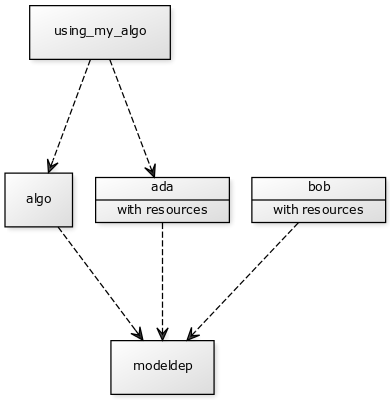
\includegraphics[width=200pt]{res/packaging_version_A.png}
\caption{Packaging Version A}
\label{fig:pkgsysA}
\end{figure}


\subsubsection{Version B}

The second approach is based on Maven's version string: an \id{algo} will depend on an abstract \id{model} which provide a mechanism to load a specific file from its jar archive and both \id{ada} and \id{bob} model versions are defined as subversion of \id{model}. For example, the convention could be that if \id{model} is defined as version \id{0.1} then \id{ada} will use the string \id{0.1-ADA} to define its version and the \id{algo} will accept versions in the range $ [0.1,0.2) $.

The model actually used will be either specified at compile time (cf. \id{using.algo2}) or be selected at runtime depending on the installed packages (cf. \id{using.algo1}) as depicted on Figure \ref{fig:pkgsysB}. While this offers a great flexibility to the user designing pipelines and allows him to swap models without repackaging anything, it means that test projects cannot ensure the correctness of more than one model version at a time. Moreover, if no specific version is bound to the pipeline, such as with \id{using.algo1}, then there is no strong guarantee that a valid version is available at runtime.

\begin{figure}
\centering
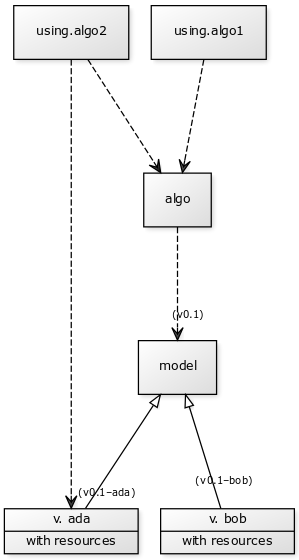
\includegraphics[width=200pt]{res/packaging_version_B.png}
\caption{Packaging Version B}
\label{fig:pkgsysB}
\end{figure}


\subsubsection{Version C}

The third version we studied is the most simple one: as illustrated on Figure \ref{fig:pkgsysC}, instead of splitting everything in separate package, only annotators are packaged independently of pipelines and resources, which are grouped together. On the one hand this system couldn't be simpler but on the other, since pipelines often involve several engine annotators that are themselves used in several pipelines, the coupling of models and the corresponding algorithm implies that many packages have to be created to support each combination of models.


\begin{figure}
\centering
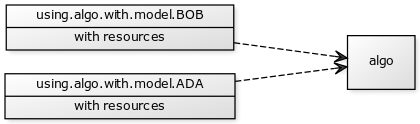
\includegraphics[width=200pt]{res/packaging_version_C.png}
\caption{Packaging Version C}
\label{fig:pkgsysC}
\end{figure}

\subsubsection{The verdict - Version D}

After exploring possibilities offered by the Maven packaging system we analysed how resources and engines are related to each others and used by pipelines in bluima. Figure \ref{fig:pkgsysD} depicts those relations. It was also considered that repackaging is an acceptable cost to swap models. The most important point was avoiding at all cost to package an exponentially huge number of pipelines to match each and every possible combinations and for this reason version C was discarded.

We also reflected on the structure of the algorithm, especially on their input arguments. We came to the conclusion that, mostly for flexibility, they should accept \id{InputStream}s as input and not be bound to any models. Instead, the pipelines will be in charge to give them the proper resource data streams. Therefore the pipeline will have dependencies toward algorithms and models.

Finally, in order to centralise code and simplify loading resources we introduce \id{ModelProxy}, a utility class used by pipelines that, given a String representing a class name, opens a stream to a given file inside the class' jar archive.

In some cases, when processing the resource as a stream, it can be convenient to have access to its original filename (e.g. when reading a compressed archive). Therefore we encapsulate the name and the stream in a class -- \id{ModelStream} -- that can be seen as a specialised \id{InputStream} with a filename property.

\begin{figure}
\centering
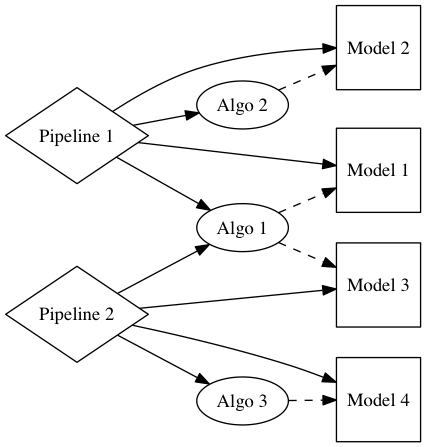
\includegraphics[width=200pt]{res/packaging_version_D.png}
\caption{Packaging Version D}
\label{fig:pkgsysD}
\end{figure}


\subsection{Restructuring bluima}
\label{sec:restructuring_bluima}

\TODO{better explain strategy before details}

Now that the packaging strategy for annotators and their resources has been designed we can actually apply it. It was decided to start with a relatively easy annotator -- namely \id{SentenceAnnotator} which is part of OpenNLP -- to make sure our previous decision was indeed viable. The approach was based on an iterative process that can be applied to other modules as well. However, let's first take a step back and discuss the file hierarchy and how the different modules are related to each others.

\subsubsection{File Hierarchy}

We wanted to create a structured, yet flexible, file hierarchy for the annotators and their resources. Since we are using Maven, we based our design on parent-child relationship in the \id{pom.xml} files: the root pom file, in addition to actually loading its children, defines the main settings, such as the Java version to use or the list of general dependencies, that will be shared with every of its children. The root pom file references both modules \path{modules/pom.xml} and \path{resources/pom.xml} that are responsible for loading their own children, that is the different annotators or utilities for the former and the actual resource for the latter.

It follows that when running the install (or test) command on the root Maven project then every algorithms and resources are installed (or tested).

\subsubsection{Case Study: Converting OpenNLP}

When converting an annotator such as \id{SentenceAnnotator}, the first thing to do is to identify the unit test responsible for its quality \TODO{add details on unit test in §bluima/§sherlok}. In this case, the annotator was imported from UIMA \TODO{ref} and it was still based on the XML engine descriptor \TODO{ref} \TODO{add explanation/contrast between XML engine descriptor \& java code in §bluima}. Therefore, we first have to make it compatible with the new and compact pipeline runner from uimaFIT \TODO{ref}.

Once the unit tests are properly working, we move on to the generation of the resource packages. Since this phase is completely repetitive, we devised a script \TODO{ref to wiki} to make the developer live less cumbersome: given a resource file, a resource name and a few other technical details we can produce a resource package, as described previously, that is ready to be used with an annotator.

However, many annotators are currently using Java \id{File} parameters, or Java \id{String}s pointing to a local file. Therefore, we have to refactor these annotators and their dependencies in order to use \id{ModelStream} instead. The following strategy was applied to convert PoS, Token and Chunk annotator of OpenNLP:

\begin{enumerate}

\item Renaming the \id{PARAM\_MODEL\_FILE} parameter (or any similar properties) of the annotator into \id{PARAM\_MODEL}.

\item Updating its \id{initialize} method to load a \id{ModelStream} through \id{ModelProxy} and the \id{PARAM\_MODEL} parameter.

\item Updating the annotator's dependencies such that they can be constructed from \id{ModelStream}. Usually this plays well with the current implementation that must at some point use a \id{FileInputStream}. Hence, we can plug in our custom stream in place of the regular \id{FileInputStream} without restructuring the dependencies too much.

\item Updating the dependency list in the annotator's \id{pom.xml} file to reflect any additional resource dependency.

\end{enumerate}

Finally, at this last point the unit test should be updated to use resource package instead of absolute path to the resource file with \id{PARAM\_MODEL}.

\subsection{Pipeline Configuration in Sherlok}

\TODO{explain how this gets configured in Sherlok}

\section{Packaging: a better approach}

\TODO{find better title}

\TODO{split into subsections maybe; git submodules for resources - shared by bluima/sherlok; }

Currently every single resource file is packaged in a separate jar file and there is a one-to-one mapping between a file and a \id{ModelResource}. Actually, several files can be grouped inside the same jar as long as the corresponding \id{ModelResource} classes are also in the same jar. However, this has several limitations that were either not identified during the design process or, wrongly, not considered as significantly limiting for our use case. The purpose of this proposal is to fix those limitation by proposing a new packaging strategy for resources.

It has been decided that, with \id{ModelResource}, we shall use \id{InputStream} instead of \id{File} and therefore refactor some code in bluima. We initially guessed that this refactoring would in practice not be a large issue because, at some point, we need to read the file -- using \id{FileInputStream} or alike -- and therefore could use a more abstract concept (\id{InputStream} vs \id{File}) without much trouble. Unfortunately, for some annotators this task is actually hard or even impossible. This is particulary true for annotators using external code, where sometime \id{File} or even \id{String} paths to resources are used. For example, the linnaeus annotator is an annotator that wraps the external Linnaeus library. This library uses an \id{ArgParser} that cannot be created from a data stream, but requires \TODO{XXX}. Hence, the only working solution that works without refactoring the (external) linnaeus library is to extract the configuration file into a temporary directory and provide the path to this temporary directory to the Linnaeus library.

Attempting to convert \id{LinnaeusAnnotator} also highlighted another issue: its main configuration file makes references to some other files with relative paths. The issue here is that with our resource packaging system the files are only accessible through streams via \id{ModelProxy} but not paths.

Here there are two potential solutions:

\begin{itemize}

\item either we completely rewrite Linnaeus, since it is a closed source program to support reference to \id{ModelResource} in the configuration files;

\item or we put all the related configuration files in an archive -- say, a tar file -- and extract them in a temporary directory.

\end{itemize}

Obviously the first solution is not practical within the short time period allocated to this project and not sustainable in the long term, as it would require to fork and constantly update the forked codebase. The second solution, however, could be achieved. It moreover solves (partially) a more general issue discussed below.

Like with \id{LinnaeusAnnotator}, the \id{BrainRegionPipes} uses a batch of files: a collection of configuration files used to set up an annotator or its dependencies. For the \id{BrainRegionPipes} the problem is easier since no file makes a reference to another one. Nevertheless, it would be very verbose and painful to load each of the ~30 files from its corresponding \id{ModelRessource}. Moreover, with our former approach we would need to add as many configuration parameters to the annotator as the number of resources it uses to make it completely independent of any version of its resources. Hence, considering a batch of files simply as a collection of resource files is not optimal.

We see two other alternatives:

\begin{enumerate}

\item First, if we devise a strict naming convention for each \id{ModelResource} class involved in setting up an annotator, then we can ask the user for a unique package name -- instead of a potentially numerous \id{ModelResource} class names -- and load each resource class from that package. While this solution is simple on the paper it actually requires as much refactoring as the naive idea previously mentioned. Additionally, it doesn't solve the issue illustrated above with \id{LinnaeusAnnotator}.

\item Alternatively, if we consider that all the files used to configure an engine have names following a precise naming specification, then we could aggregate them in an archive that would get extracted at runtime in a temporary directory. This solution has at least two significant advantages:

\begin{itemize}

\item it requires only a minimal rewrite of the current Java code to extract and use the data,

\item and it allows files to refer to one another through relative paths.

\end{itemize}

\end{enumerate}

A bluima user such as Sherlok could specify which temporary directory should be used instead of a default one -- say, \path{/tmp} -- through an extra configuration parameter so that he can manage the lifetime of the extracted data. However, with or without this extra parameter, the system would make things relatively complicated for the system administrator. For example, when installing annotation tools the user cannot know beforehand how much disk space is needed. But more importantly this would imply adding a relatively complex version checking system in bluima: in order to not extract when it is already available to prevent degrading performance we would have to check if the data is actually correct. This can be quite complex when, for example, upgrading the resources. And this is without mentioning having several pipelines using the same engine but with different version of its resources, nor dealing with multiple concurrent annotation instances. Finally, if we take the example of Sherlok running on several servers, we have the issue of data accessibility and replication for cache purposes.

In addition to all the above issues, we could argue that we actually remove flexibility from the user by forcing him to use a Java system to archive and manage resources despite the fact that the system using bluima could be Java agnostic from the final user point of view. It could actually be quite painful for someone who is using a SCM (source control management, e.g. git or svn) such as git to manage two distinct files structures: one that is convenient to the user and one for our jar archiving system.

Moreover, at the end of the day, we have extracted some data that the user had to package initially in order to make the installation process easy. But this installation process could have been much simpler: instead of all those intermediary steps the user could have simply installed the configuration files on a directory of his own. From the bluima's perspective, since this simpler approach does not enforce any versioning mechanism at all, the user is free to implement any system that matches his needs. Following from this fact, Sherlok can add an extra layer -- potentially directly integrated in the bundle configuration file -- to manage resources easily for the end user. Such system could (but is not restricted to) be based on git: a user would define a (batch of) resource(s) with a git repository and either a tag or a commit SHA and Sherlok would automatically download and install the specific version of the resources.

This last solution allies the flexibility of using Java \id{File} objects -- and therefore does not necessitate any refactoring of bluima annotators -- with the power of external, well-establish and powerful SCM tools in addition to avoid the limitation of having to rely solely on \id{InputStream} to access resources.

\subsection{Restructuring bluima}

\TODO{write me}

\subsection{Pipeline Configuration in Sherlok}

\TODO{write me}

\subsubsection{Configuration Variables}

\TODO{write me}

\section{Future Work}

\TODO{ideas? support for more variable url pattern (svn, ...) }
\TODO{overview figure, e.g.  Sherlok's Linnaeus bundle, that downloads the bluima Maven jar (that itself depends on the Linnaeus Maven library) and the Linnaeus config file; Sherlok's Linnaeus pipeline that uses them to annotate species}
%\newpage
%\begin{appendix}
%  \listoffigures
%  \listoftables
%\end{appendix}

\end{document}
